\documentclass[serif,mathserif]{beamer}
\usepackage{amsmath, amsfonts, epsfig, xspace}
\usepackage{algorithm,algorithmic}
\usepackage{pstricks,pst-node}
\usepackage{multimedia}
\usepackage{pdfpages}
\usepackage[normal,tight,center]{subfigure}
\setlength{\subfigcapskip}{-.5em}
\usepackage{beamerthemesplit}
\usetheme{lankton-keynote}

\author[Kamal Lamichhane]{Kamal Lamichhane }

\title[ECE-254, Lab 2A\hspace{2em}\insertframenumber/\inserttotalframenumber]{LAB TUTORIALS-2A}
\subtitle[] {Operating System and System Programming-ECE254}


\date{Sept 15, 2016} %leave out for today's date to be insterted

\institute{Electrical and Computer Engineering, University of Waterloo, University of Waterloo}

\begin{document}

\maketitle

% \section{Introduction}  % add these to see outline in slides

\begin{frame}{Who am I? }
\begin{itemize}
    \item MASc Student in the ECE Department
    \item Working in the area of Real-time Embedded Software Systems
    \end{itemize}
 \end{frame}
 
 \begin{frame} {When and Where to find me ?}
 \begin{itemize}
     \item E5-5122 
     \item kamal.lamichhane@uwaterloo.ca 
     \item www.lamichhanekamal.com.np \pause
     \item Office time - Learn, Calander in the website: www.lamichhanekamal.com.np/Cal.pdf \pause
     \item Drop an email if you need assistance any other time
     
 \end{itemize}
 
  \end{frame}

\begin{frame}
  \frametitle{Introduction}
  Task Management in ARM RL-RTX\pause
  \begin{itemize}
  \item Read kernel task control block related data structure (PART-A)\pause
  \item Block and unblock a task by using context switching related kernel functions (Part-B)\pause
  \item Memory Management \pause %leave out the \pause on the final item \pause
  \item NOTE :: Lab2/starter: Two files are changed from original source code of Keil so that the return value in TCB is changed to U32. Remember to include modified HAL\_CM3.c and rt\_Typredef.h. \pause
  \item main\_task\_exp.c- Subroutine to map a function pointer address to the function name.
  \end{itemize}
\end{frame}

\begin{frame}
  \begin{itemize}
  
  
      \item Stay Hungry. Stay Foolish. --- Get your thinking clean to make it simple...
      
  \end{itemize}
\end{frame}



 \section{Project} % add these to see outline in slides
 
 

\begin{frame}
  Answer the questions from lab manual 2.4.1.
\end{frame}

\begin{frame}
  \frametitle{Programming Project Part-A}
  \begin{figure}
    \centering
    
\includegraphics[width=10cm]{abc.jpg}
  \end{figure}
\end{frame}


\begin{frame}
   \frametitle{What you have to do?}
   You are to implement a primitive to obtain
the task status information from the RTX at runtime given the task id.

\begin{itemize}
    \item  OS\_RESULT  os\_tsk\_get (OS\_TID task\_id, RL\_TASK\_INFO *buffer)
\end{itemize}
\end{frame}

\begin{frame} [label=firstframe]
\frametitle{Programming Project Part-A}
   The primitive returns information about a task. The system call returns a rl\_task\_info
structure , which contains the following fields: \pause
  \begin{figure}
    \centering
    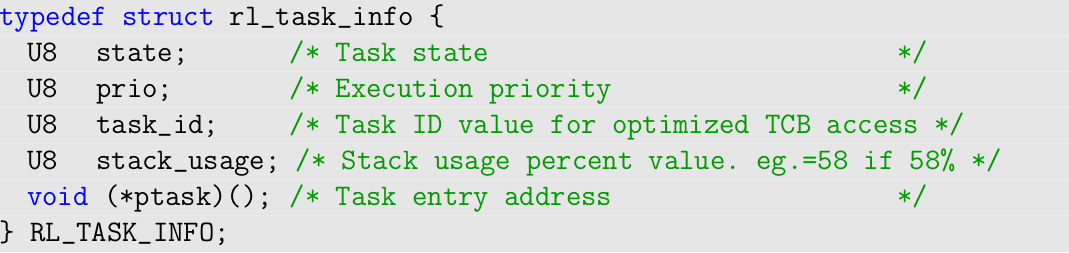
\includegraphics[width=12cm]{sc.png}
  \end{figure}
\end{frame}


\begin{frame}
\frametitle{Programming Project Part-A}
STATES: \pause
\begin{itemize}
    \item Inactive -Tasks which have not been started or deleted
\item Ready - Tasks which are ready to run
\item Runnning - Task that is currently running
\item Wait\_dly - Tasks which are waiting for a delay to expire.
\item Wait\_sem - Tasks which are waiting for a semaphore
\item Wait\_mut -Tasks which are waiting for a free mutex
\item Wait\_mbx - Tasks which are waiting for a mailbox message 
 \item Wait\_mem - Tasks which are waiting for memory
\end{itemize}
\end{frame}




\begin{frame} [label=firstframe]
\frametitle{Programming Project Part-A}
  \begin{figure}
    \centering
    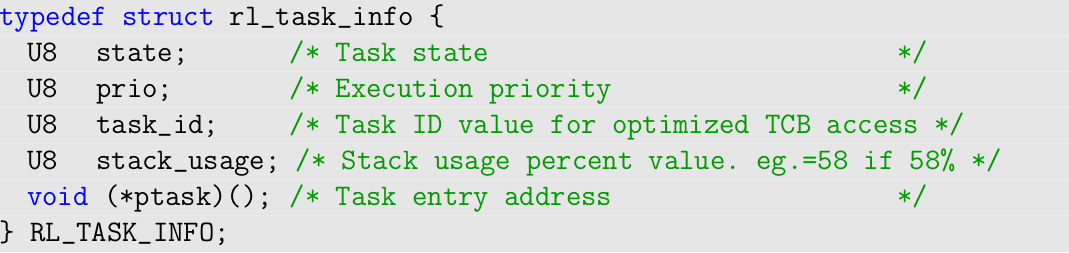
\includegraphics[width=12cm]{sc.png}
  \end{figure}
\end{frame}

\begin{frame}
\frametitle{Programming Project Part-A}

\begin{itemize}
\item The prio field describes the priority of this task.
\item The task\_id field describes the id of task assigned by the OS.
\item  The stack\_usage describes how much stack space is used by this task. The value is
the percent value. For example, if 58\% of this task stack is used, stack\_usage is set
to 58.
\item The ptask field describes the entry address of this task function.
 \item The function returns OS\_R\_OK on success and OS\_R\_NOK otherwise.
\end{itemize}
\end{frame}

\begin{frame} {Deliverables}
Submit a compressed archive file that contains the following:
\begin{enumerate}
\item A lab2\_QA.txt file which contains answer to questions in Section 2.4.1.
\item Your entire multi-project workspace to solve the programming project.
\item A test description file to describe what each testing task does. Name the file Test\_spec.txt.
\item A README file to describe what you have submitted and how to build and run your
project(s).
\end{enumerate}
  
\end{frame}

\begin{frame} {Note}
\begin{itemize}
\item  Please Follow Source Code File Organization Convention.
\item Check Third party testing in lab manual 2.4.4
\end{itemize}
  
\end{frame}







\begin{frame}
  \frametitle{Questions}
  
  Review Lecture 1, 2, and 3.
  \begin{enumerate}
  \item Introduction
  \item Review of Computer Architecture 
  \item Operating system Structure and Traps
  \end{enumerate}
\end{frame}
\end{document}
